\RequirePackage[l2tabu, orthodox]{nag}
\RequirePackage{ifxetex}
\RequireXeTeX
\documentclass{article}

%颜色
\usepackage{xcolor}
\xdefinecolor{lightBlue}{rgb}{.22,.45,.7}
\xdefinecolor{darkGrey}{rgb}{.45,.45,.45}
\xdefinecolor{DeepSkyBlue}{RGB}{0, 104, 139}
\xdefinecolor{dkpurple}{rgb}{.455, .204, .506}

%长度
\usepackage{printlen}
\uselengthunit{mm}

%图形
\usepackage{media9}
\usepackage{pdfpages}
\usepackage{overpic}
\usepackage{graphicx}
\graphicspath{{./src/}}
\usepackage{wallpaper}
\usepackage{wrapfig}
\usepackage{pstricks}
\usepackage{tikz}
\usetikzlibrary{patterns}
\usetikzlibrary{arrows}
\usetikzlibrary{shapes}
\usetikzlibrary{chains}
\usetikzlibrary{mindmap}
\usetikzlibrary{graphs}
\usepackage{scsnowman}
\usepackage{tikzpeople}
\usepackage{tikzducks}
\usepackage{pifont}
\usepackage{marvosym}
%\usepackage{bbding}
%\usepackage{SIunits}
\usepackage{stmaryrd}
\usepackage{ean13isbn}
\newcommand{\drawbarcode}[1]{\EANisbn[SC5a, ISBN = #1]}
\usepackage{qrcode}

%%进度条
\newcommand{\progressbar}[2][2cm]{%
	\textcolor{lightBlue}{\rule{#1 * \real{#2} / 100}{1.5ex}}%
	\textcolor{darkGrey!15}{\rule{#1 - #1 * \real{#2} / 100}{1.5ex}}
}

%表格
\usepackage{tabu}
\usepackage{longtable}
\usepackage{booktabs}
\usepackage{diagbox}
\usepackage{multicol}
\usepackage{multirow}
\usepackage{makecell}
\usepackage{fancybox}
\usepackage{colortbl}
\usepackage[minted]{tcolorbox}
\tcbuselibrary{skins}
\tcbuselibrary{breakable}
\tcbuselibrary{theorems}
\tcbuselibrary{listings}
\tcbuselibrary{xparse}
\usepackage{fvextra}
\usepackage{csvsimple}
\usepackage{siunitx}

%公式
\usepackage{amsmath}
\usepackage{amsthm}
\usepackage{amsfonts}
\usepackage{amssymb}
\usepackage{amsbsy}
\usepackage{amsopn}
\usepackage{amstext}
\usepackage{mathrsfs}
\usepackage{bm}
\usepackage{textcomp}
\usepackage{latexsym}
\usepackage{exscale}
\usepackage{relsize}
%\usepackage{xymtex}

%正文
\usepackage{fancyhdr}
\usepackage{geometry}
\usepackage{lastpage}
\usepackage{indentfirst}
\usepackage{setspace}
\renewcommand\arraystretch{1.5}
\renewcommand{\thefootnote}{\fnsymbol{footnote}}

%非正文
\usepackage{makeidx}
\makeindex
\usepackage{epigraph}
\usepackage{varwidth}

%%链接
\usepackage
[	colorlinks = true,
linkcolor = gray,
citecolor = gray,
backref=page
]{hyperref}
\usepackage{caption}
\usepackage{subcaption}
\DeclareCaptionLabelFormat{andtable}%
{#1#2~\&~\tablename\thetable}
%\renewcommand{\thetable}{\alph{table}}
%\renewcommand{\thefigure}{\Alph{table}}
%\renewcommand{\thesubtable}{\Roman{subtable}}
%\renewcommand{\thesubfigure}{\arabic{subfigure}}
%\captionsetup[figure]{labelfont=it,textfont={bf,it}}
%\captionsetup[subfigure]{labelfont=bf,textfont=normalfont,singlelinecheck=off,justification=raggedright}

%其它
\usepackage{atbegshi}
\newcommand{\handlethispage}{}
\AtBeginShipout{\handlethispage}
\usepackage{lipsum}

%枚举%与beamer冲突
\usepackage{enumitem}
\setlist[enumerate, 1]
{	fullwidth,
	label = \arabic*.,
	font = \textup,
	itemindent=2em
}

%\endofdump

\bibliographystyle{IEEEtran}
%\usepackage[notref,notcite]{showkeys}

%中文
\usepackage{ctex}
%\xeCJKsetup{
%	CJKecglue = {\hskip .10em plus .05em minus .05em},
%	CheckSingle = true
%}
%\setCJKmainfont[
%	BoldFont = {Noto Serif CJK SC Bold},
%	ItalicFont = {AR PL UKai HK}
%]{Noto Serif CJK SC ExtraLight}
%\setCJKsansfont[
%	BoldFont = {Noto Sans S Chinese Medium},
%	ItalicFont = {Noto Sans S Chinese DemiLight}
%]{SimSun}
%\setCJKmonofont[
%	BoldFont = {Adobe Heiti Std},
%	ItalicFont = {Adobe Kaiti Std}
%]{WenQuanYi Micro Hei Mono Light}
%\setCJKfamilyfont{zhkesong}{MF KeSong (Noncommercial)}
%\setCJKfamilyfont{zhhjsd}{MF TheGoldenEra (Noncommercial)}
%\setCJKfamilyfont{zhlangsong}{MF LangSong (Noncommercial)}
%\newcommand{\hjsd}{\CJKfamily{zhhjsd}}
%\newcommand{\KeSong}{\CJKfamily{zhkesong}}
%\newcommand{\langsong}{\CJKfamily{zhlangsong}}
%\newfontfamily\KeSongf[Mapping = tex-text]{MF KeSong (Noncommercial)}
%\newfontfamily\hjsdf[Mapping = tex-text]{MF TheGoldenEra (Noncommercial)}
%\newfontfamily\langsongf[Mapping = tex-text]{MF LangSong (Noncommercial)}
%\newfontfamily\SourceCodePro[Mapping = tex-text]{Source Code Pro}
%\newfontfamily\monaco{Monaco}
%\usepackage{microtype}

%%代码
\usepackage{minted}
%Java %与mcode冲突
% \usepackage{lstcustom}
%Matlab %与lstcustom冲突
%\usepackage[framed,numbered,autolinebreaks,useliterate]{mcode}
\usepackage{boxie}
\makeatletter
\xdefinecolor{tcbcol@back}{rgb}{0,0,0}
\makeatother
\renewcommand*\lstlistingname{代码}

\title{\textbf{非线性电阻电路的应用\\——混沌电路}}
\author{}
\date{}

%页眉页脚%与book冲突
\pagestyle{fancy}
\renewcommand{\headrulewidth}{0pt}
\lhead{}
\chead{}
\rhead{}
\lfoot{\small{第\chinese{section}节}}
\cfoot{\small{第\thepage 页~共~\pageref{LastPage}~页}}
\rfoot{}
\usepackage{titlesec}
%\titleformat{\chapter}{\centering\Huge\bfseries}{实验\chinese{chapter}~}{4mm}{}
\titleformat{\section}{\large\bfseries}{\chinese{section}、}{1mm}{}
\titleformat{\subsection}{}{\arabic{subsection}.}{1mm}{}
\titleformat{\subsubsection}{}{(\arabic{subsubsection})}{1mm}{}
\begin{document}

\begin{titlepage}
	\centering
	\begin{figure}[htbp]
		\centering
		\includegraphics[width=.8\linewidth]{NJUST.ai}
		\label{fig:NJUST}
	\end{figure}

	\vspace{20mm}
	\textbf{\zihao{1}\heiti{电工电子}}

	\vspace{5mm}
	\textbf{\zihao{1}\heiti{综合实验论文}}

	\vspace{20mm}
	\begin{table}[htbp]
		\centering
		\zihao{3}
		\begin{longtabu}to.8\linewidth{@{}X[4,r]@{}X[c]@{}X[12,l]@{}}
			\makebox[4\ccwd][s]{学院}&:&\underline{\makebox[12\ccwd][c]{\kaishu{电子工程与光电技术学院}}}\\
			\makebox[4\ccwd][s]{班号}&:&\underline{\makebox[12\ccwd][c]{\kaishu{9171040G11}}}\\
			\makebox[4\ccwd][s]{姓名}&:&\underline{\makebox[12\ccwd][c]{\kaishu{吴振宇}}}\\
			\makebox[4\ccwd][s]{学号}&:&\underline{\makebox[12\ccwd][c]{\kaishu{916101630117}}}
		\end{longtabu}
	\end{table}

	\vspace{10mm}
	\zihao{3}
	\kaishu{\today}
\end{titlepage}

\maketitle

\begin{abstract}
	本文以能产生混沌行为的最简的一种自治电路—蔡氏电路为基础,在multisim14.0的平台上用一个非线性负电阻电路设计一个混沌电路,在Octave5.1.1.0的平台上编制程序对非线性电阻度伏安特性曲线进行了绘制,研究了蔡氏电路在不同参数下的混沌现象。从理论分析和仿真两个角度分别研究蔡氏电路中的混沌现象。

	两个负阻抗变换器并联可以实现非线性电阻,并以此为渠道得到蔡氏混沌电路。

	在计算机辅助条件下,可以以很高精确度完成模拟元件的伏安特性曲线测量和绘制。

	在实验中发现了混沌电路确实存在敏感参数,在参数渐变时,呈现出明显的混沌现象。

	让人们从感性上更加清晰地了解混沌现象产生的机理,熟悉混沌现象产生的条件,掌握电路中混沌状态的基本规律,使人们对电路中的混沌现象具有更具体、更形象的认识。
\end{abstract}

\textbf{关键词:非线性电阻;蔡氏电路;混沌现象;Multisim14.0仿真。}

\newpage

\section{引言}%
\label{sec:引言}

混沌(Chaos)是20世纪物理学的重大事件。混沌研究最先起源于洛伦兹研究天气预报时用到的三个动力学方程。后来的研究表明,无论时复杂的系统,如气象系统、太阳系,还是简单系统,如滴水龙头等,皆因存在着内在随机性而出现类似无轨,但实际是非周期有序运动,即混沌现象。现在混沌研究涉及的领域包括数学、物理学、生物学、化学、天文学、经济学及工程技术的众多学科,并对这些学科的发展产生了重要影响,混沌包含的物理内容非常广泛,研究这些内容更需要比较深入的数学理论,如微分动力学方程、拓补学、分形几何学等。目前混沌的研究重点已转向多维动力学系统中的混沌、量子及时空混沌、混沌的同步及控制等方面。电路中存在混沌现象已经是在理论和实验中证明了的不争的事实。

二十多年来混沌一直是举世瞩目的前沿课题和研究热点它揭示了自然界及人类社会中普遍存在的复杂性有序与无序的统一确定性与随机性的统一大大拓宽了人们的视野加深了对客观世界的认识。许多人认为混沌的发现是继上世纪相对论与量子力学以来的第三次物理学革命。目前混沌控制与同步的研究成果已被用来解决秘密通讯、改善和提高激光器性能以及控制人类心律不齐等问题。

混沌科学的发展,不仅大大拓宽了人们的视野,并加深了人们对客观世界的认识,而且由于混沌的奇异特性,尤其是对初始条件微小变化的高度敏感性及其不稳定性,还促使人们思考,混沌在现实生活中到底是有害还是有益?混沌是否可以控制?它有何应用价值及其发展前景?1990年,皮卡拉和卡罗提出了混沌同步的概念,约克等人提出了混沌控制的概念,这些结论很快为实验所证实。事实上,任何事物都有二重性,混沌也不例外。一方面,对有害的混沌加以控制就是混沌控制;另一方面,对有益的混沌设法产生和加强就是混沌反控制。

蔡式电路由于具有丰富的混沌动力学特征,所以是目前实验观察最好的混沌电路之一,也是当前研究最多的一类混沌电路。该电路是由美国贝克莱大学的蔡少棠教授首先发起研究的,它是一个三阶自治电路。它是由两个电容、一个电感、一个电阻和一个非线性电阻组成,结构非常简单。混沌是发生在确定系统中的一种不确定行为.在某些三阶非线性自治电路中就存在着混沌现象,这类动态电路的方程是三阶非线性常微分方程.它的解在一定参量值下对初始条件十分敏感,容易产生混沌现象。

实现蔡氏电路的核心就是实现本实验借助非线性电阻电路。电路理论中,通常将电路划分为线性电路和非线性电路两大类。从严格意义上来讲,线性电路是不存在的,它仅仅是在特定的工作点附近呈现出所谓的“线性”特征,一旦电路的外部条件或内部参数发生变化使其偏离工作点(有时仅仅是微小的偏离),电路的线性特征将会大大地削弱,如发生信号波形失真、电路出现“噪声过量”等现象。非线性是所有电气电路、电子电路具有的固有特性。

\section{正文}%
\label{sec:正文}

\subsection{设计背景}%
\label{sub:设计背景}

蔡式电路(见图 \ref{fig:蔡氏电路})是美国贝克莱(Berkeley)大学的蔡少棠教授(Leon. O. Chua)设计的能产生混沌行为的最简的一种自治电路。该典型电路并不惟一。蔡式电路在非线性系统及混沌研究中,占有极为严重的地位。

在蔡氏电路及蔡氏振荡器的分析及实验研究中,为电路建立一个精确的试验模型,从而观察非混沌现象并定量分析它,这一点十分重要。而其中非线性电阻电路的实现是这一环节的一个关键。

\subsection{设计要求}%
\label{sub:设计要求}

利用非线性负电阻电路,设计如图\ref{fig:非线性电阻伏安特性曲线}的非线性伏安特性曲线。

在图\ref{fig:非线性负电阻设计}中,横坐标为电压,小于\SI{+-18}{V};纵坐标为电流,小于\SI{+-18}{mA}。

\begin{enumerate}
	\item 用列表法测量并作出该伏安特性曲线;
	\item 试用使用示波器观察该伏安特性曲线。
\end{enumerate}

\subsection{设计参考}%
\label{sub:设计参考}

查找资料,以上述伏安特性曲线电路为基础,设计混沌电路。

\begin{enumerate}
	\item 试用使用示波器观察该混沌电路的混沌现象(如图 \ref{fig:蔡氏电路相轨图随滑动变阻器阻值逐渐变化而变化}所示,不惟一);
	\item 改变混沌电路的敏感参数,观察记录混沌现象;
	\item 总结混沌电路的研究工作。
\end{enumerate}

\subsection{设计思路}%
\label{sub:设计思路}

蔡氏电路电阻是一个分段线性的负电阻,整体呈现对称但非线性。负电阻是出现混沌的原因。其特性至少可用三种方法来实现:

\begin{enumerate}
	\item 两个晶体管和两个二极管;
	\item 一个运算放大器和两个二极管;
	\item 一个双运算放大器和六个线性电阻组合。
\end{enumerate}

考虑到运算放大器具有放大系数高,使用方便。故选用两个运算放大器。

通过虚短、虚断容易判断运算放大器和正负反馈的电阻构成了一个负阻抗变换器。在运算放大器的两端出现的转折点,是输入超过放大器的放大区所致。所以选用2个不同的负阻抗变换器就可以实现左右各有两个折点的蔡氏电路电阻。

为了使实验结果更接近真实,设计中没有使用理想元件以便可以在实验室环境中通过真实实验检验仿真的正误。运算放大器选用了德克萨斯仪器公司的TL082,这是一种电源适用范围大、工作稳定、比较常见的运算放大器。其原理图和引脚图见图\ref{fig:TL082原理图}和\ref{fig:TL082引脚图}。

\begin{figure}[htpb]
	\centering
	\begin{subfigure}[htpb]{.45\linewidth}
		\centering
		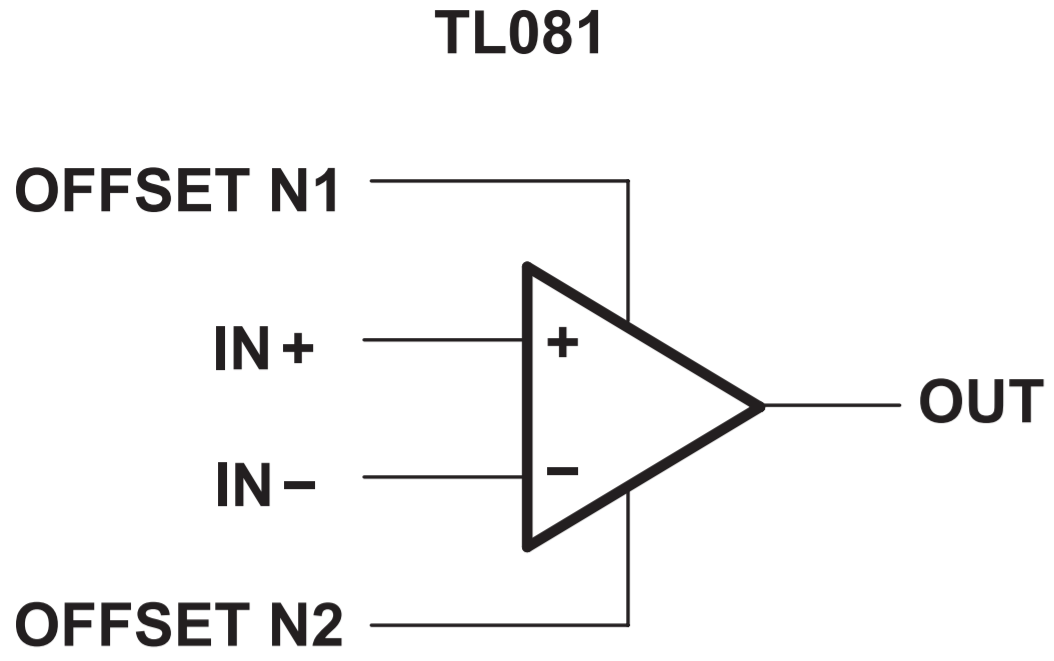
\includegraphics[width=.9\linewidth]{TL082scheme.png}
		\caption{TL082原理图}
		\label{fig:TL082原理图}
	\end{subfigure}
	\quad
	\begin{subfigure}[htpb]{.45\linewidth}
		\centering
		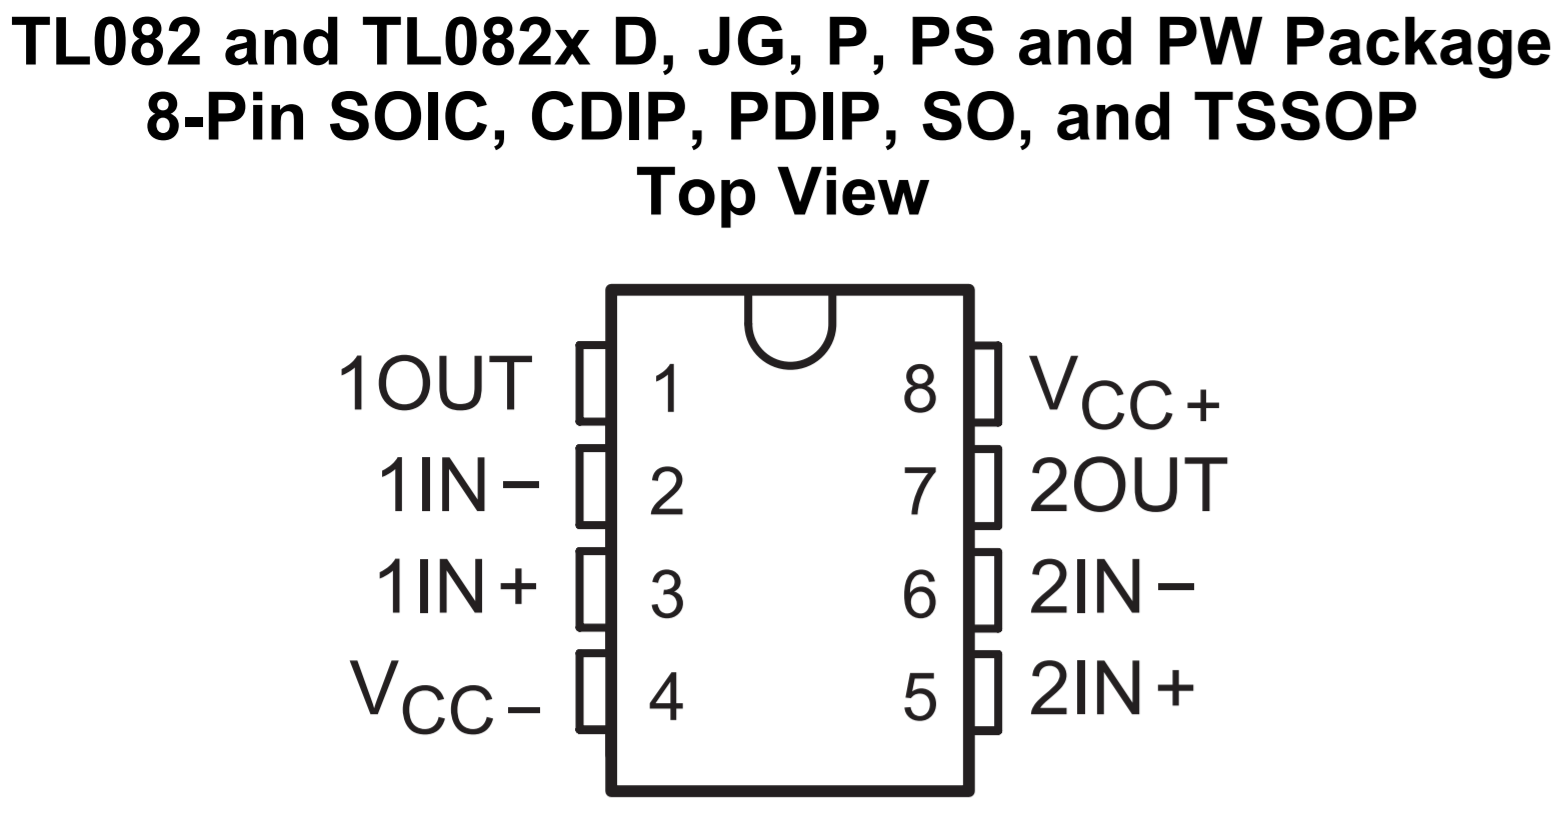
\includegraphics[width=.9\linewidth]{TL082pin.png}
		\caption{TL082引脚图}
		\label{fig:TL082引脚图}
	\end{subfigure}
	\caption{TL082原理图和引脚图}
	\label{fig:TL082原理图和引脚图}
\end{figure}

在电阻的选择上,选用了标称电阻的E24系列,如表\ref{tab:E24系列}。以方便在实际环境中找到对应阻值的电阻。

\begin{table}[htpb]
	\centering
	\caption{E24系列}
	\label{tab:E24系列}
	\csvreader[
	head to column names,
	tabular=cccccccccccc,
	table head=
	\toprule
	\multicolumn{12}{c}{E24系列:误差\SI{+-5}{\%}}
	\\
	\midrule,
	table foot=\bottomrule
	]{src/E24.csv}{}{ \a&\b&\c&\d&\e&\f&\g&\h&\i&\j&\k&\l }
\end{table}

\subsection{实验设备}%
\label{sub:实验设备}

Multisim14.0电路仿真软件中的模拟元件:

\begin{enumerate}
	\item 万用表;
	\item 运算放大器;
	\item 示波器;
	\item 直流电源;
	\item 电阻若干。
\end{enumerate}

\subsection{实验目的}%
\label{sub:实验目的}

\begin{enumerate}
	\item 通过实验感性地认识混沌现象,理解非线性科学中“混沌”一词的含义;
	\item 学会借助Multisim14.0仿真软件对电路进行研究;
	\item 掌握非线性电阻的非线性特征,以及其非线性电阻特征的测量方法;
	\item 以非线性电阻电路为基础,设计混沌电路,观察混沌现象。
\end{enumerate}

\subsection{仿真实验}%
\label{sub:仿真实验}

\subsubsection{非线性负电阻设计}%
\label{ssub:非线性负电阻设计}

\begin{figure}[htbp]
	\centering
	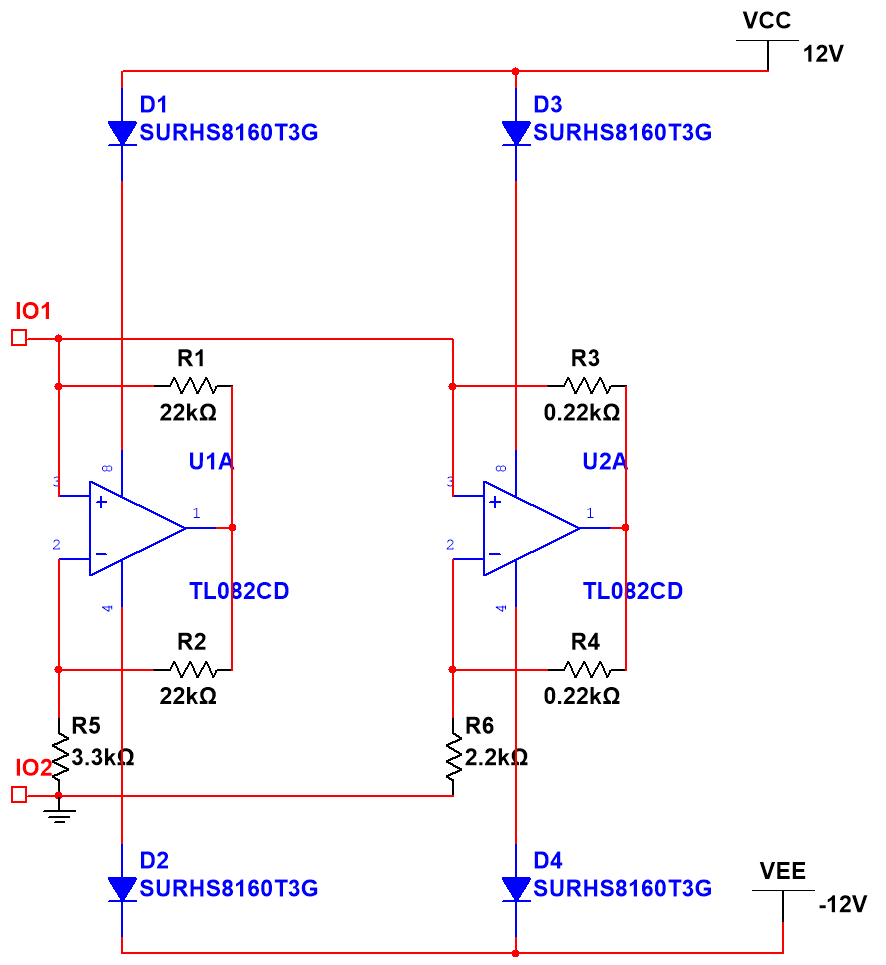
\includegraphics[width=.6\linewidth]{ChuaR0.png}
	\caption{非线性负电阻设计}
	\label{fig:非线性负电阻设计}
\end{figure}

考虑到实际电路中常有的正负极反接保护,故在电源端串联了二极管。因为该电路之后会重复利用,为了方便起见,将蔡氏电阻电路\ref{fig:非线性负电阻设计}封装成一个子电路,只留出了电阻连接的两个输入输出口。

\begin{figure}[htpb]
	\centering
	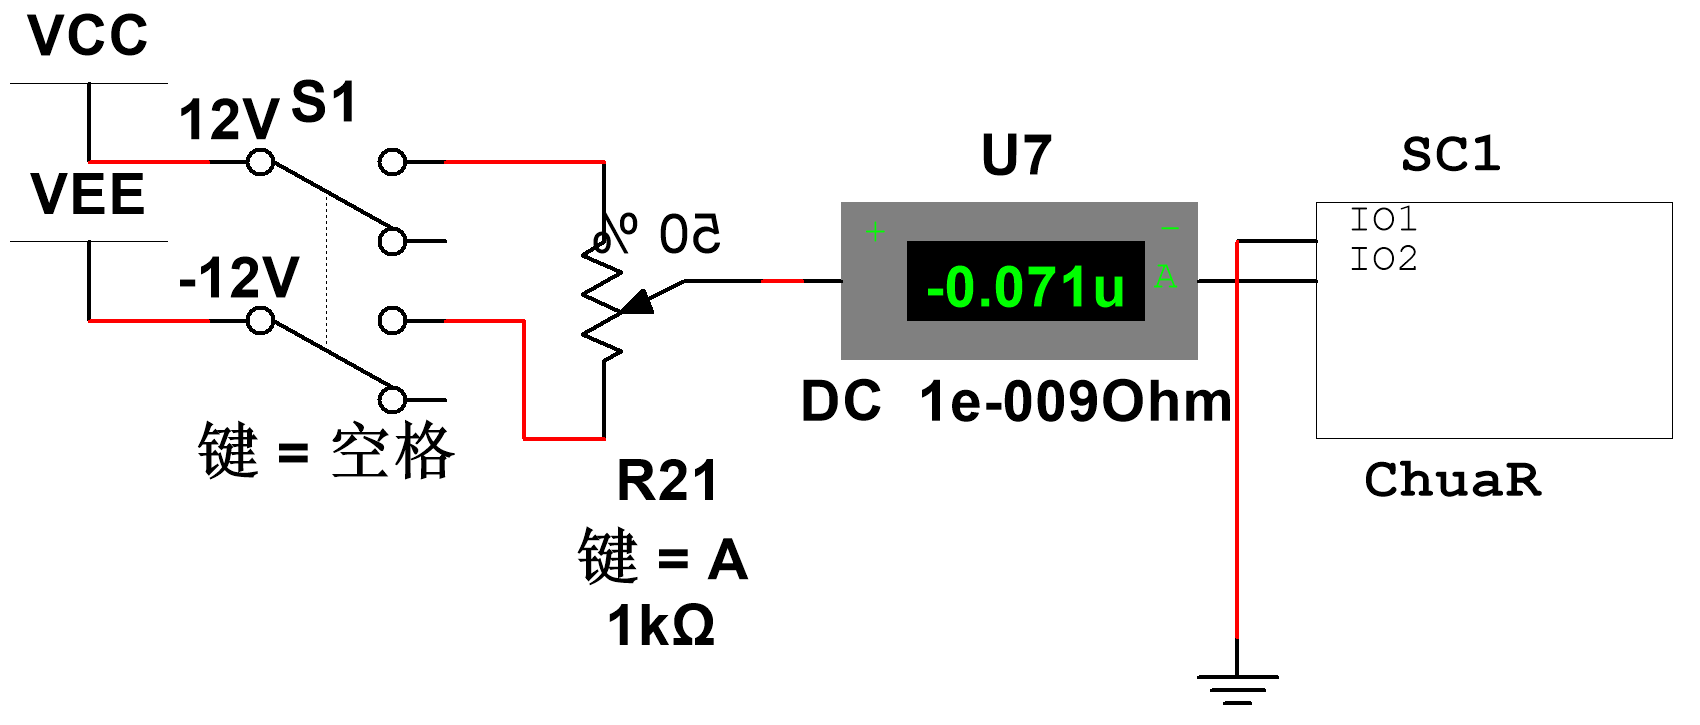
\includegraphics[width=0.7\linewidth]{ChuaR1.png}
	\caption{用伏安法测量伏安特性曲线}
	\label{fig:用伏安法测量伏安特性曲线}
\end{figure}

如图\ref{fig:用伏安法测量伏安特性曲线},滑动变阻器起着分压作用,使蔡氏电阻电路两端的电压可以在\SI{-12}{V}到\SI{+12}{V}之间自由变化。仿真开始时,闭合双刀双掷开关使电路接通,电流表就会有示数。记录此时的滑动变阻器变阻百分比和电流表示数。可得表\ref{tab:滑动变阻器变阻百分比和电流表示数关系}。为了更接近实际,电流表也选择了具有一定阻值的电流表。

\begin{table}[htpb]
	\centering
	\small
	\caption{滑动变阻器变阻百分比和电流表示数关系}
	\label{tab:滑动变阻器变阻百分比和电流表示数关系}
	\csvreader[
	head to column names,
	tabular=cccc,
	table head=
	\toprule
	滑动变阻器变阻百分比/\%&电流表示数/\SI{}{mA}&滑动变阻器变阻百分比/\%&电流表示数/\SI{}{mA}
	\\
	\midrule,
	table foot=\bottomrule
	]{src/ChuaR.csv}{}{ \a&\b&\c&\d }
\end{table}

\newpage

接下来对数据进行处理以得到蔡氏电阻电路的伏安特性曲线。程序源码如程序清单\ref{fig:数据处理程序源码}所示。每一步的意图见注释。

\begin{figure}[htpb]
	\centering
	\langCVfile[Octave][fig:数据处理程序源码][Octave]{./src/ChuaR.m}{src/ChuaR.m}
	\caption{数据处理程序源码}
\end{figure}

\newpage

运行界面如图\ref{fig:运行界面}。

\begin{figure}[htpb]
	\centering
	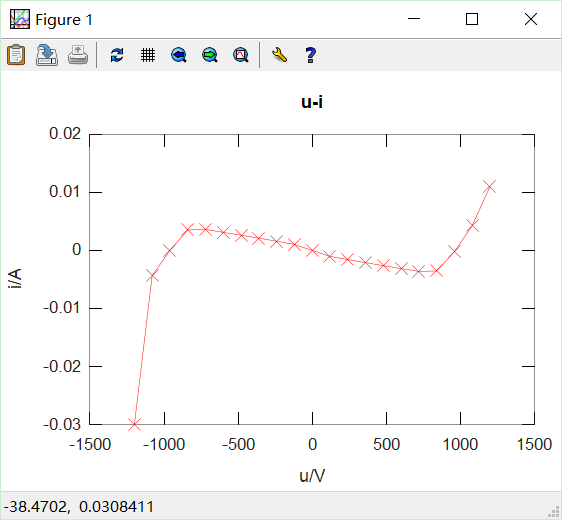
\includegraphics[width=0.6\linewidth]{ChuaRm.png}
	\caption{运行界面}
	\label{fig:运行界面}
\end{figure}

运行结果如图\ref{fig:程序运行结果},用时稍长是因为保存文件的操作。

\begin{figure}[htpb]
	\centering
	\winlightfile{Octave-5.1.1.0}{src/ChuaR.txt}
	\caption{程序运行结果}
	\label{fig:程序运行结果}
\end{figure}

\newpage

即便是使用程序辅助绘图,列表法仍需部分手动操作,稍显繁琐。在使用示波器的情况下,测量伏安特性曲线的过程可以更加方便。

\begin{figure}[htbp]
	\centering
	\begin{subfigure}[htbp]{.45\linewidth}
		\centering
		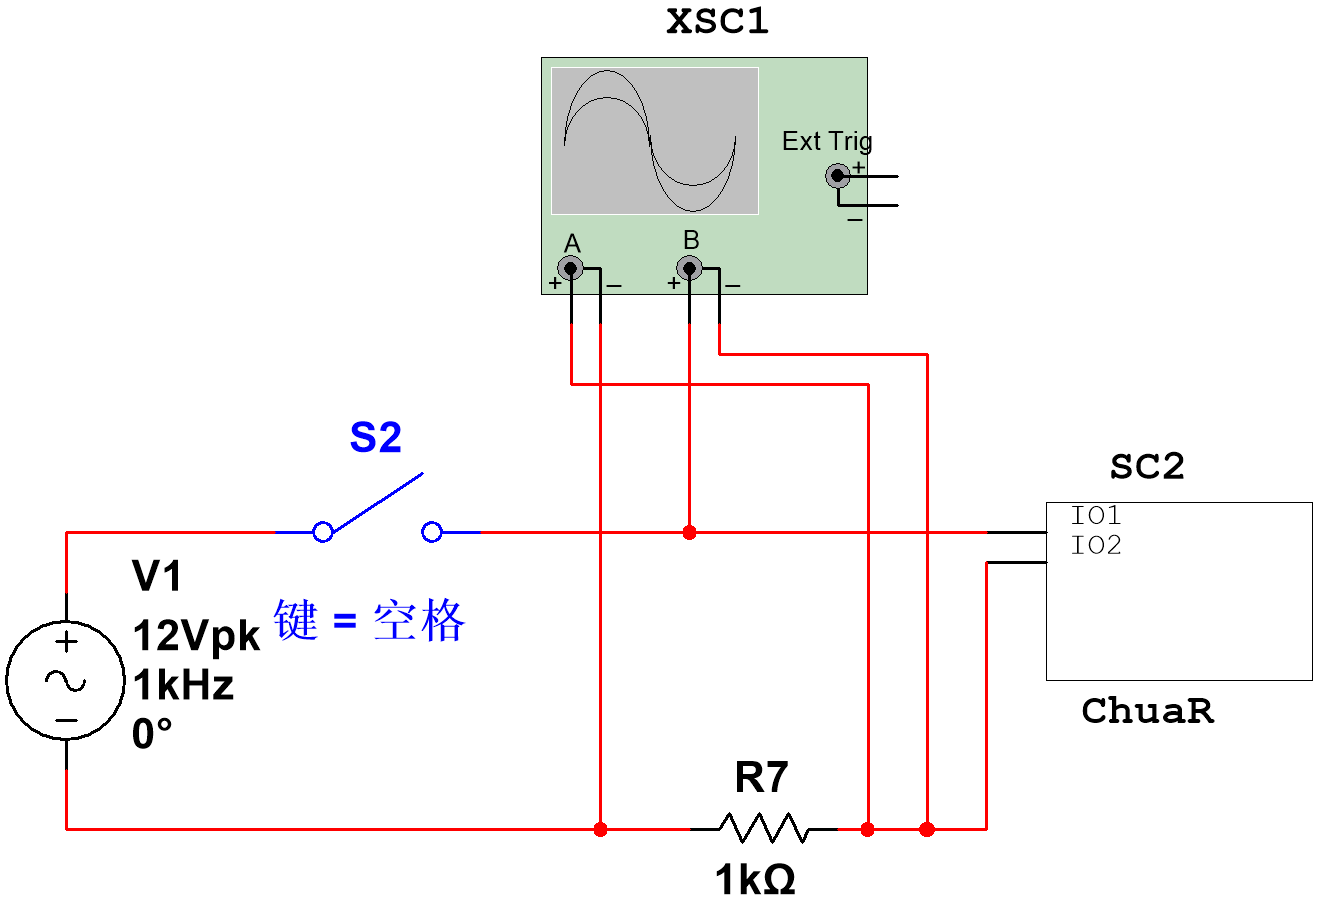
\includegraphics[width=\linewidth]{ChuaR2.png}
		\caption{用函数电源测量伏安特性曲线}
		\label{fig:用函数电源测量伏安特性曲线}
	\end{subfigure}
	\quad
	\begin{subfigure}[htbp]{.45\linewidth}
		\centering
		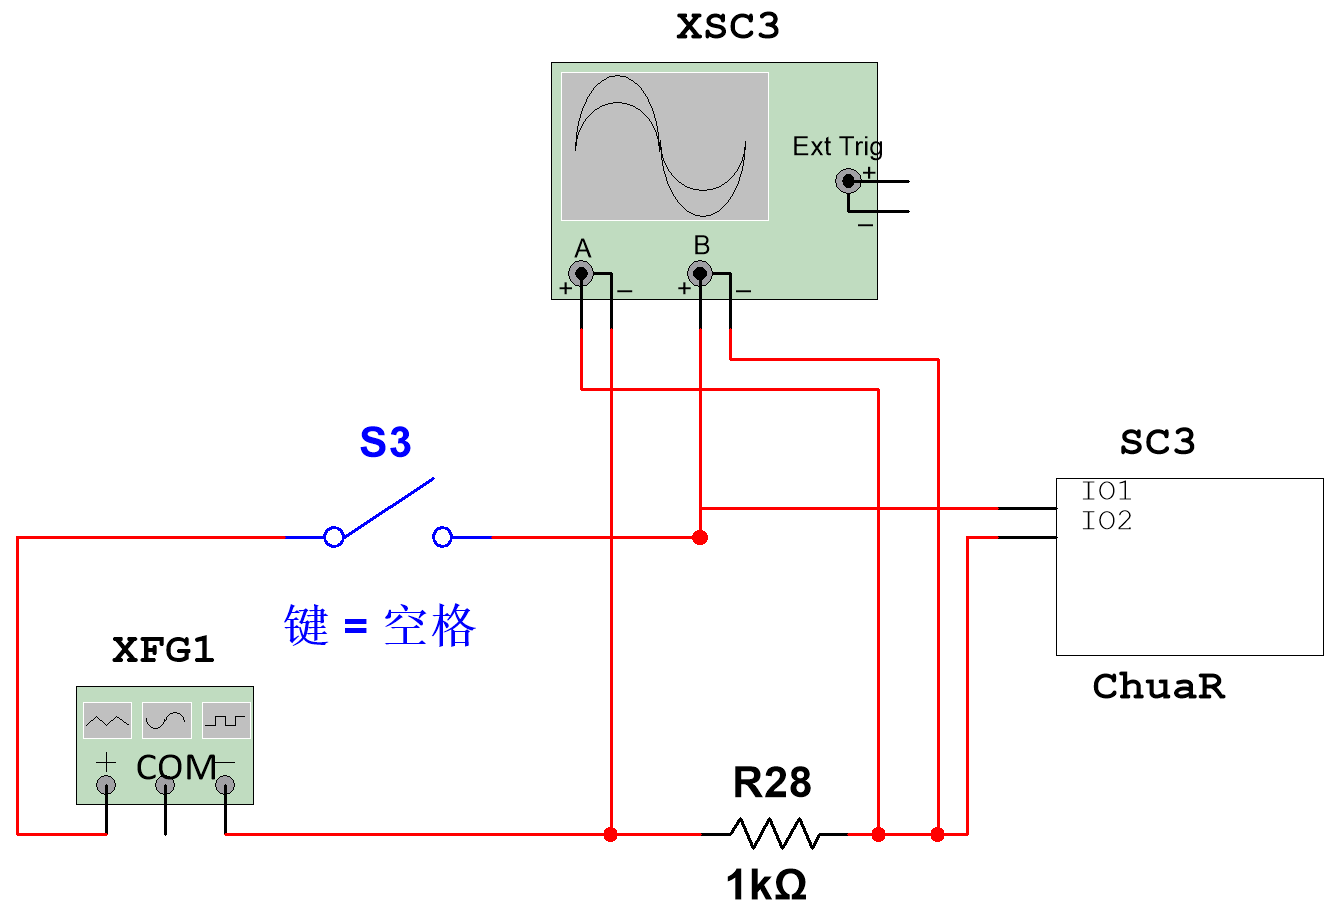
\includegraphics[width=\linewidth]{ChuaR3.png}
		\caption{用交流电压源测量伏安特性曲线}
		\label{fig:用交流电压源测量伏安特性曲线}
	\end{subfigure}
	\caption{测量伏安特性曲线的2种方法}
	\label{fig:测量伏安特性曲线的2种方法}
\end{figure}

如图\ref{fig:用函数电源测量伏安特性曲线}和\ref{fig:用交流电压源测量伏安特性曲线},图中示波器一端输入信号为蔡氏电阻电路两端电压,另一端输入信号为\SI{1}{k\ohm},因为电阻的伏安特性曲线为线性,所以蔡氏电阻电路电流即为该电阻的电压除以\SI{1}{k\ohm}。值得注意的是电压变化频率不宜过快,例如函数信号发生器输出方波信号的话,变化频率过快就不能显示连续的伏安特性曲线了。利用示波器可以直接查看伏安特性曲线,也可输出scp文件以便后续使用程序进行数据处理和辅助绘图。

\begin{figure}[htbp]
	\centering
	\begin{subfigure}[htbp]{.30\linewidth}
		\centering
		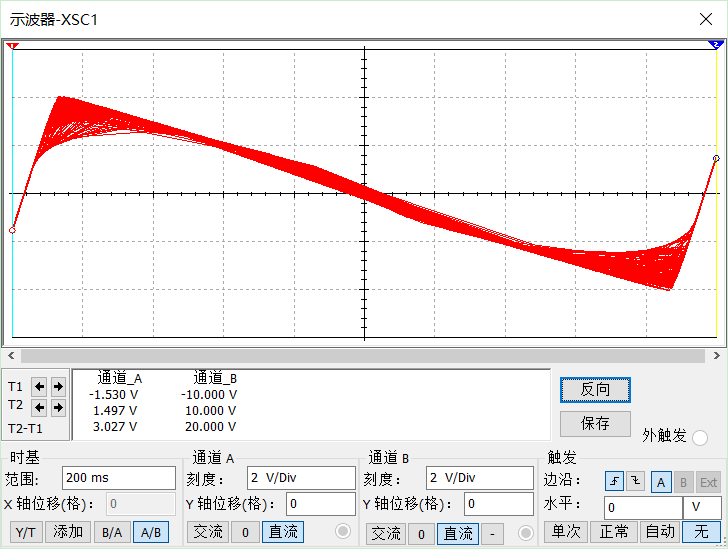
\includegraphics[width=\linewidth]{ChuaVA1.png}
		\caption{非线性电阻伏安特性曲线测量范围内边界值}
		\label{fig:非线性电阻伏安特性曲线测量范围内边界值}
	\end{subfigure}
	\quad
	\begin{subfigure}[htbp]{.30\linewidth}
		\centering
		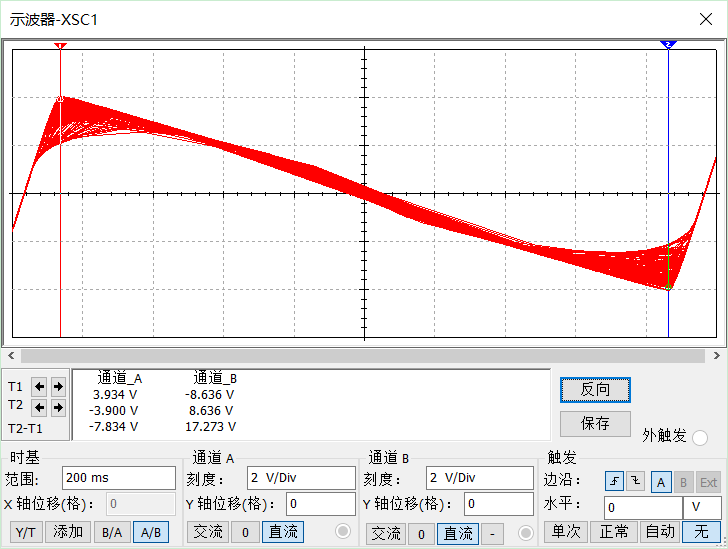
\includegraphics[width=\linewidth]{ChuaVA2.png}
		\caption{非线性电阻伏安特性曲线极值点}
		\label{fig:非线性电阻伏安特性曲线极值点}
	\end{subfigure}
	\quad
	\begin{subfigure}[htbp]{.30\linewidth}
		\centering
		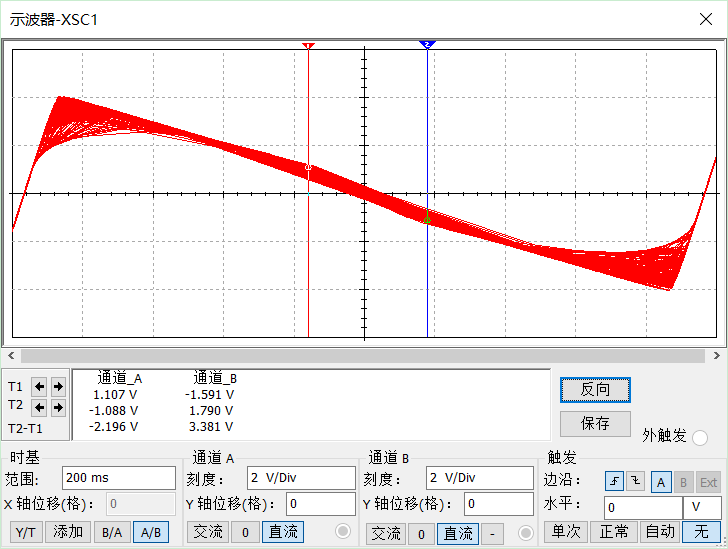
\includegraphics[width=\linewidth]{ChuaVA3.png}
		\caption{非线性电阻伏安特性曲线离原点最近的转折点}
		\label{fig:非线性电阻伏安特性曲线极值点离原点最近的转折点}
	\end{subfigure}
	\caption{非线性电阻伏安特性曲线}
	\label{fig:非线性电阻伏安特性曲线}
\end{figure}

\newpage

实际上如果选用电流电压分析仪的话可以更加方便。如图\ref{fig:用电流电压分析仪测量伏安特性曲线}。

\begin{figure}[htpb]
	\centering
	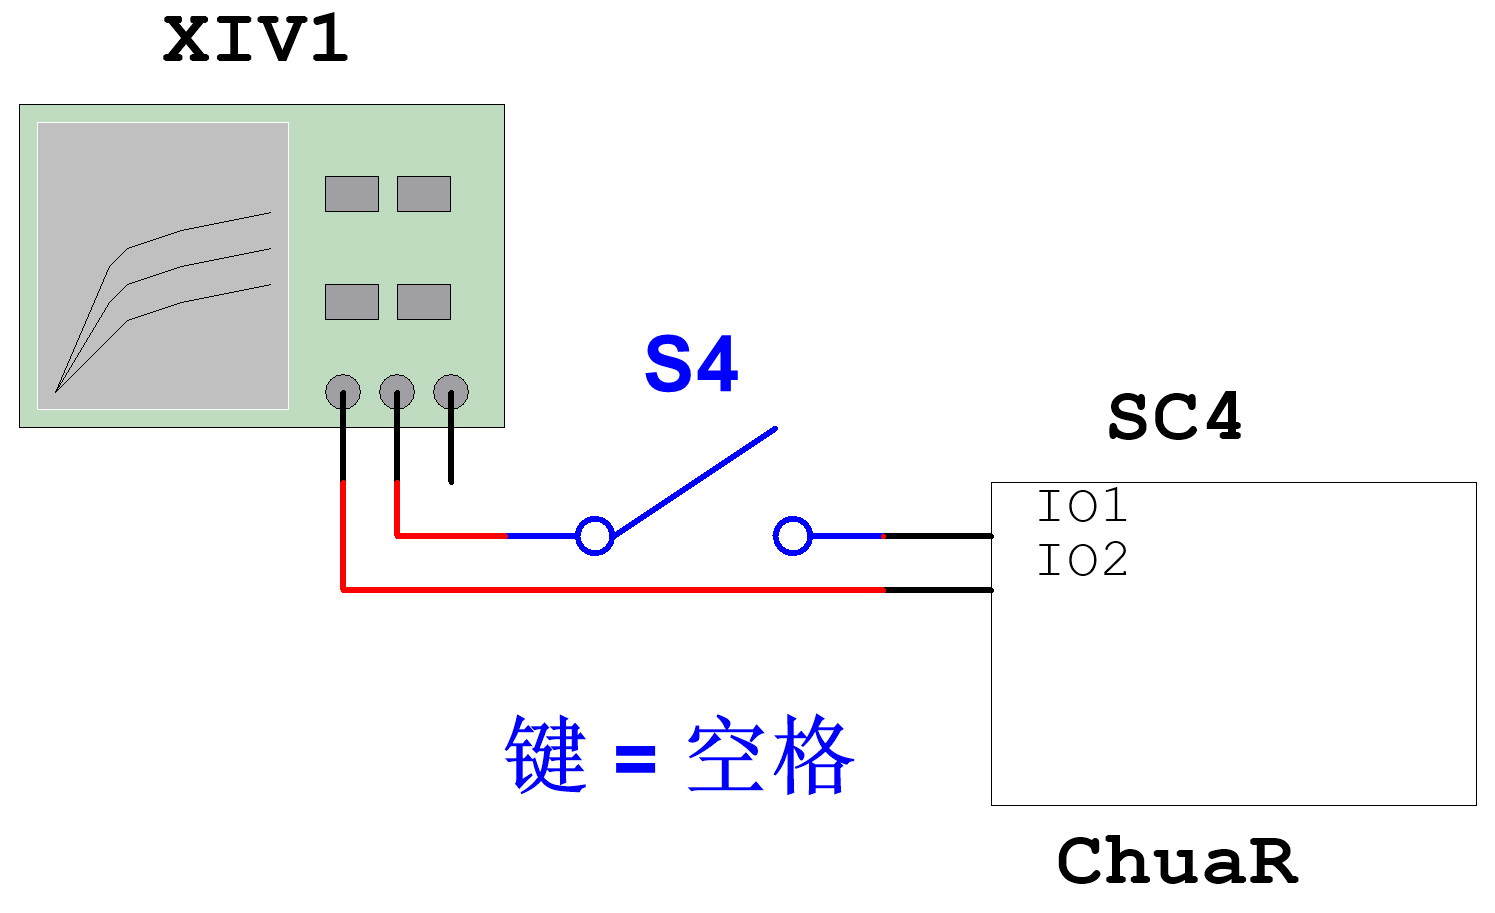
\includegraphics[width=.4\linewidth]{ChuaR4.png}
	\caption{用电流电压分析仪测量伏安特性曲线}
	\label{fig:用电流电压分析仪测量伏安特性曲线}
\end{figure}

\subsubsection{蔡氏电路相轨图分析}%
\label{ssub:蔡氏电路相轨图分析}

利用蔡氏电阻电路就可以设计如图\ref{fig:蔡氏电路}所示的蔡氏电路。蔡氏电路是一个典型的混沌电路。电路中的电感\( L \) 和电容\( C_1 \) 并联构成一个振荡电路。\( R_{Chua} \) 是一个有源非线性负电阻元件,电感\( L \) 和电容\( C_2 \) 组成一损耗可以忽略的谐振回路;可变电阻\( R_{14} \) 和电容\( C_2 \) 串联将振荡器产生的正弦信号移相输出。

\begin{figure}[htbp]
	\centering
	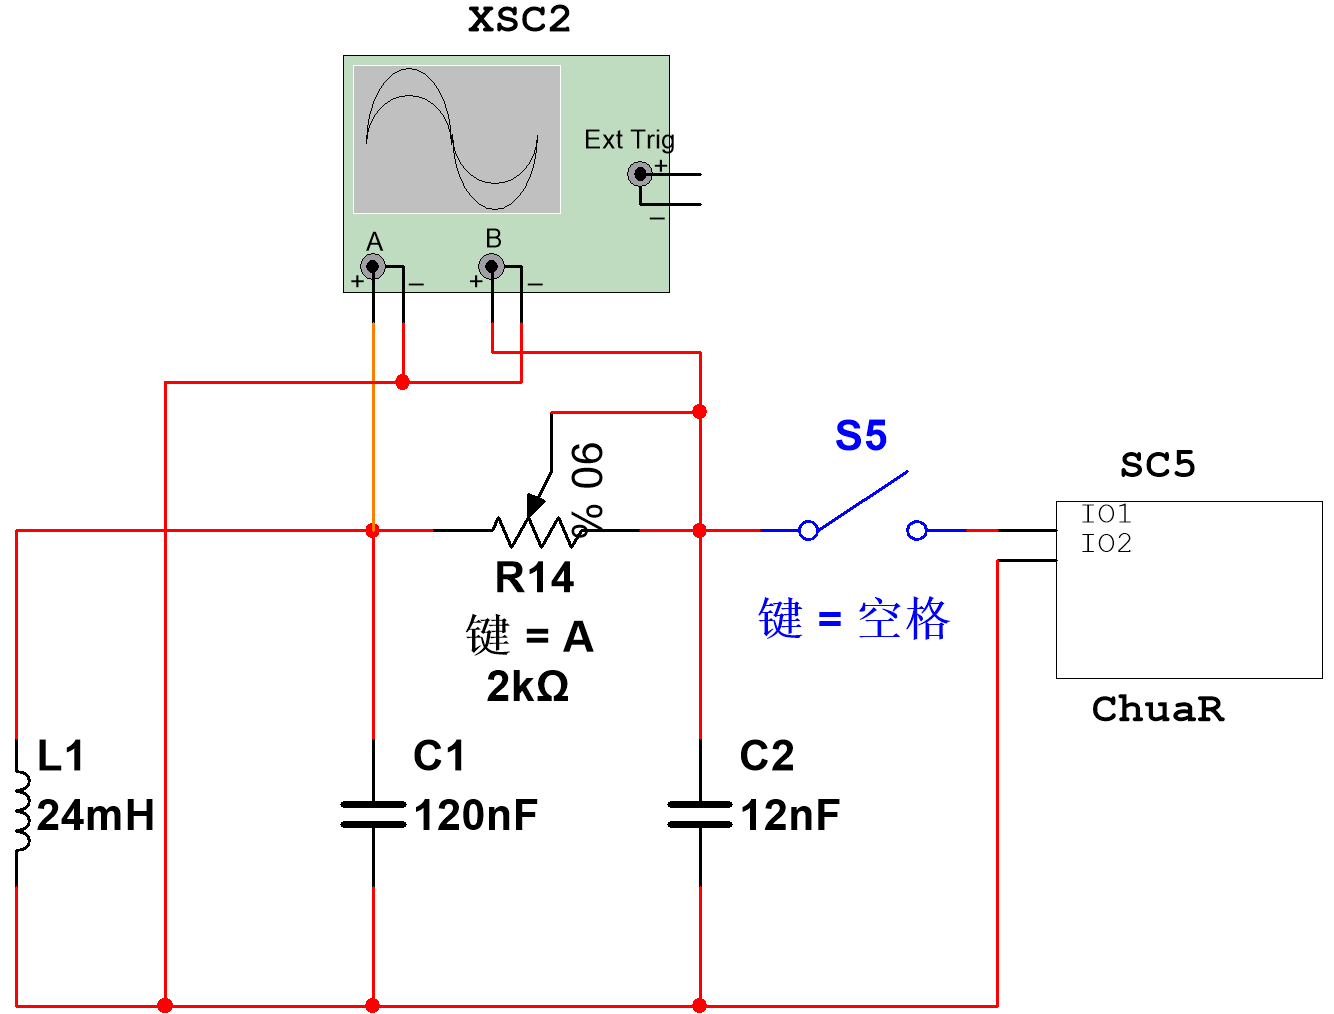
\includegraphics[width=.5\linewidth]{ChuaR5.png}
	\caption{蔡氏电路}
	\label{fig:蔡氏电路}
\end{figure}

\newpage

利用状态方程分析法根据蔡氏电路的特性树写出该电路的状态方程。特性树为\( C_1,R_{14},C_2 \)。对树枝上的电容列写节点电压方程,对连枝上的电感列写路电路方程,得到状态方程组\ref{eq:状态方程}。该方程没有解析解。

\begin{align}
	\left\{
		\begin{array}{lcl}
			C_1\dfrac{\mathrm{d}}{\mathrm{d}t}U_{C_1}&=&\dfrac{U_{C_2}-U_{C_1}}{R_{14}}- \dfrac{U_{C_1}}{R_\mathrm{Chua}}
			\\
			C_2\dfrac{\mathrm{d}}{\mathrm{d}t}U_{C_2}&=&\dfrac{U_{ C_{1} }-U_{ C_{2} }}{R_{14}}+i_{L}
			\\
			L\dfrac{\mathrm{d}}{\mathrm{d}t}i_L&=&-U_{C_{2}}
			\label{eq:状态方程}
		\end{array}
	\right.
\end{align}

逐步改变滑动变阻器变阻百分比,观察\( C_1,C_2 \) 相轨图。

\newcommand{\mypng}[2]{
	\begin{subfigure}[htbp]{.45\linewidth}
		\centering
		\includegraphics[width=.9\linewidth]{Chua#1.png}
		\caption{滑动变阻器变阻百分比为#2}
		\label{fig:滑动变阻器变阻百分比为#2}
	\end{subfigure}
}

\begin{figure}[htbp]
	\centering
	\mypng{0}{0}
	\quad
	\mypng{10}{10}

	\mypng{20}{20}
	\quad
	\mypng{30}{30}
\end{figure}

\begin{figure}[htbp]
	\begin{subfigure}[htbp]{0\linewidth}
	\end{subfigure}

	\setcounter{subfigure}{4}

	\mypng{40}{40}
	\quad
	\mypng{50}{50}

	\mypng{60}{60}
	\quad
	\mypng{70}{70}

	\mypng{80}{80}
	\quad
	\mypng{100}{100}
	\caption{蔡氏电路相轨图随滑动变阻器阻值逐渐变化而变化}
	\label{fig:蔡氏电路相轨图随滑动变阻器阻值逐渐变化而变化}
\end{figure}

\newpage

示波器屏上先是可以观察到一条直线,调节R7,直线不断变宽,逐渐成为类似椭圆的图像。最终漩涡中心从一个变成两个并向中心轴两边扩展形成双吸引子。此时环状曲线在两个向外涡旋的吸引子之间不断填充与跳跃,这就是混沌研究文献中所描述的“蝴蝶”图像,是一种整体上的稳定性和局域上的不稳定性同时存在的奇异吸引子。

在滑动变阻器变阻百分比为90\%时情况会比较特殊。如图\ref{fig:蔡氏电路相轨图随滑动变阻器阻值从正负两个方向变化}所示,从0\%逐步增大到90\%的相轨图和从100\%逐步减小到90\%的相轨图是不一样的。

\begin{figure}[htbp]
	\centering
	\mypng{90from80}{90,从负方向趋向}
	\quad
	\mypng{90from100}{90,从正方向趋向}
	\caption{蔡氏电路相轨图随滑动变阻器阻值从正负两个方向变化}
	\label{fig:蔡氏电路相轨图随滑动变阻器阻值从正负两个方向变化}
\end{figure}

进一步修改阻值,发现逐步增加时蔡氏电路在84\%会出现混沌吸引子\footnote{混沌吸引子:吸引子是指这样的一个集合,当时间趋于无穷大时,在任何一个有界集上出发的非定常流的所有轨道都趋于它。若吸引子的轨线对初始条件高度敏感依赖,该吸引子就称为混沌吸引子。吸引子无外乎两种状态,即单个点和稳定极限环。系统的吸引子理论是关于吸引子的科学理论,它是混沌学的重要组成部分。奇异(怪)吸引子:具有分数维结构的吸引子称为奇异吸引子。奇异吸引子是反映混沌系统运动特征的产物,也是一种混沌系统中无序稳态的运动形态。它具有自相似性,同时具有分形结构。奇异吸引子是混沌运动的主要特征之一。奇异吸引子的出现与系统中包含某种不稳定性(不同于轨道不稳定性和李雅普诺夫不稳定性)有着密切关系,它具有不同属性的内外两种方向:在奇异吸引子外的一切运动都趋向(吸引)到吸引子,属于“稳定”的方向;一切到达奇异吸引子内的运动都互相排斥,对应于“不稳定”方向。},而逐步减小时则在98\%会出现混沌吸引子。如图\ref{fig:参数相同的蔡氏电路相轨图对初值的灵敏度极高}所示,这说明参数相同的蔡氏电路相轨图对初值的灵敏度极高。

\begin{figure}[htbp]
	\centering
	\mypng{83}{83}
	\quad
	\mypng{84}{84}

	\mypng{85}{85}
	\quad
	\mypng{99}{99}

	\mypng{98}{98}
	\quad
	\mypng{97}{97}
	\caption{参数相同的蔡氏电路相轨图对初值的灵敏度极高}
	\label{fig:参数相同的蔡氏电路相轨图对初值的灵敏度极高}
\end{figure}

\newpage

\section{总结}%
\label{sec:总结}

本实验是在参照前人研究成果的基础上做的。实验中所要求的非线性负电阻电路并不唯一,而本实验所选用的以两个运算放大器和六个配置电阻的形式来实现是其中最简单的一种电路,本实验通过使用Multisim14.0仿真软件加以调试得到了如上的波形,所得实验结果与要求基本符合。在实验的过程中在图书馆和互联网上查阅了大量的资料,对各类参数之间的关系有了一定的了解,对非线性负电阻及混沌现象的产生有了进一步的了解和认识。

混沌至今没有统一的定义, 但人们一致的看法是: 一个确定的非线性系统, 如果含有貌似噪声的有界行为, 且又表现若干特性, 便可称为混沌系统, 此处所说的若干特性主要是如下三个方面:

\begin{enumerate}
	\item 振荡信号的功率连续分布,且可能是带状分布的,这个特征表明振荡为非周期的,也就是说明信号貌似噪声的原因;
	\item 在相空间,该系统的相邻近的轨道线彼此以指数规律迅速分离,从而导致对初始值得极端敏感性,这使得系统的行为长期不可预测;
	\item 在轨道线存在的相空间的某一特定的有界部分内,轨道线具有遍历性和混合性。遍历性是指任何一条轨道线会探访整个特定的有界部分,混合性是指初始间单关系将弥漫的动力学行为所消除。
\end{enumerate}

混沌具有两个基本的特征:一是运转状态的非周期性,即混沌系统输出信号的周期为无穷大,且在功率上与纯粹噪声信号难以分辨,因而是随机信号,然而混沌系统是确定性动力学系统,本身并不包含任何随机因素的作用,其产生随机输出信号的原因完全是因为系统内部各变量之间的强非线性耦合。因此,其输出的随机信号在理论上是可以精确重复的。二是对初始条件的高度敏感性,即若存在对初始条件的任何微小的偏离(扰动),则此偏离随着系统的演化将迅速以指数率增长,使得在很短的时间内系统的状态与受扰前便失去任何的相关性,因此,混沌仅具有极为短期的预测性。混沌状态具有以下三个关键(核心)概念:即对初始条件的敏感性、分形、奇异吸引子。

混沌作为一个科学概念,是指一个确定性系统中出现的类似随机的过程。理论和实验都证实即使是最简单的非线性系统也能产生十分复杂的行为特性,可以概括一大类非线性系统的演化特性。混沌现象出现在非线性电路中是极为普遍的现象

许多非线性动力系统的特性曲线不是跟踪简单、有规则和可预测的轨线,而是围绕像随机且似乎不规则但是明确的形式滑动。只要有关的过程是非线性的,甚至简单的严格确定性的模型可能发展这样复杂的行为。这行为被理解或接受为混沌,而且它已经导致非线性科学和动力系统工程的惊人发展。混沌理论是近年来国际上兴起的新理论,它广泛应用于电路系统,并具有很强的抽象性,不容易被接受.

混沌现象表现了非周期有序性,看起来似乎是无序状态,但呈现一定的统计规律,其基本判据有:

\begin{description}
	\item[频谱分析:]\( R_{14} \) 很小时,系统只有一个稳定的状态(对应一个解),随\( R_{14} \)的变化系统由一个稳定状态变成在两个稳定状态之间跳跃(两个解),即由一周期变为二周期,进而两个稳定状态分裂为四个稳定状态(四周期,四个解),八个稳定状态(八周期,八个解)等,直至分裂进入无穷周期,即为连续频谱,接着进入混沌,系统的状态无法确定,分岔是进入混沌的途径;
	\item[稳定性:]无穷周期后,由于产生轨道排斥,系统出现局部不稳定;
	\item[奇异吸引子存在:]奇异吸引子有一个复杂但明确的边界,这个边界保证了在整体上的稳定,在边界内部具有无穷嵌套的自相似结构,运动是混合和随机的,它对初始条件十分敏感。
\end{description}

随着计算机和计算科学的快速发展,混沌现象及其应用研究已成为自然科学技术和社会科学研究领域的一个热点。而非线性电路是混沌及混沌同步应用研究的重要途径之一,其中一个最典型的电路是三阶自治蔡氏电路。在这个电路中观察到了混沌吸引子。蔡氏电路是能产生混沌行为最简单的自治电路,所有从三阶自治常微分方程描述的系统中得到的分岔和混沌现象都能够在蔡氏电路中通过计算机仿真和示波器观察到。经过若干年的研究及目前对它的分析,无论是在理论方面、模拟方面还是实验方面均日臻完善。在理论和实践不断取得进展时,人们也不断开拓新的应用领域,如在通信、生理学、化学反应工程等方面不断产生新的技术构想,并有希望很快成为现实。

基于混沌电路的特性,它在许多领域中有重要的应用。但由于目前混沌学仍处于研究阶段,故其应用并不完善,出现的一些问题还有待解决。

\begin{description}
	\item[保密通信中的应用:]通信在我们的生活中的作用越来越重要 , 尤其是电子商务的兴起,对保密通信提出了更高的要求。利用混沌进行保密。通信是现在十分热门的研究课题。

		混沌信号最本质的特征是对初始条件极为敏感,并导致了混沌信号的类随机特性。用它作为载波调制出来的信号当然也具有类随机特性。因而,调制混沌信号即使被敌方截获,也很难被破译,这就为混沌应用于保密通信提供了有利条件。因此利用混沌进行保密通信是目前十分热门的研究课题。混沌信号最本质的特征是对初始条件极为敏感,并由此信号又具有整体稳定性 , 当我们用同一个混沌信号去驱动两个相同的系统时,两个系统的某些部分将产生同步化的行为,这就为混沌应用于保密通信提供了可行性。

		使强度更大的混沌信号和真实信号同步,由于混沌信号具有信号频谱宽、类似噪声、随机不可预测等特性,当真实信号被混沌信号所掩盖时,攻击者就很难从传输信号中分离出原始真实信号。另外要求收发两端使用相同的混沌系统以及系统参数和状态初值,使系统同步并输出相同的混沌信号,以便正确地恢复信号;
	\item[自动控制中的应用:]考察非线性混沌系统的输出信号与输入信号的自反馈耦合,或者从系统外部强迫注入某一周期信号,或者直接将系统自身的输出信号取出一部分经过一定的时间延迟后再反馈到原混沌系统中去。作为控制信号,通过调节控制因子及控制信号的大小实现稳定控制;
	\item[传感应用:]混沌具有初值敏感性,当其结构参数稳定时,初始值与动力轨道在一定的时间内是一一对应的,而且对于微小的初值变化,其运动轨迹就会出现指数分离。若初值细微变化是由混沌系统中的传感元件随被测参数变化而引起的,则轨迹之间的巨大差异就能直接反映被测参数的大小。这种混沌型传感器具有很高的灵敏度和分辨率,特别适用于微应变、微应力的测量;微量变化物参数的测量。
	\item[心脏生理学]倍周期分岔产生的混沌有可能帮助心律不齐、心肌梗塞这些医学难题找到正确的答案。
\end{description}

就目前形势而言,对混沌理论有所了解的人并不多,而事实上,混沌与人类生存环境间的关系却极其密切,混沌学的进步不仅将进一步解释那些尚未为人所知的东西,而且还孕育着一场深刻的科技革命,已涉及的学科有电子、天文、气象、激光、机械、化学、生物、医学、信息经济甚至音乐艺术等。预期的混沌应用范围涉及疾病的混沌诊断与混沌医疗、混沌控制与混沌制导、混沌通信、混沌振荡以及混沌在农业生产中的应用。我们有理由相信,混沌理论及其应用研究必将促使社会生产力的巨大发展。

\section{收获}%
\label{sec:收获}

通过本次实验,我逐步掌握了Multisim的一些基本操作。虽然我更喜欢使用simulink,但multisim在电路仿真方面比较专精,而且能和美国仪器公司的LabVIEW有机结合。而simulink不光电路仿真,包括控制仿真、数学模型也都面面俱到,并能通过用matlab编写s-function的形式利用matlab丰富的函数库。可以说两个软件各有所长。将来我将利用它们优越的仿真性能方便我今后的学习生涯。

在本次实验中,我收获颇多。因为电工实验感觉误差有点大,担心会影响成绩,所以决定好好做一下这个电路仿真实验。在看了许多资料之后发现这些课题其实原理都不复杂,电路也基本没有什么难点。最终决定选择混沌电路只是单纯觉得这个对数学的要求可能会高一点,也许会对我兴趣。动力系统涉及到的数学很深,而工科基本以应用为主,都是能用就行,不强求深入了解原理。导致更多是知其然而不知其所以然。我希望以后如有机会能更加深入地学习。

这篇论文除了使用multisim仿真外,还使用vim编辑、tex排版、Octave绘图。经过这番经历,我感觉我对计算机的了解更加深入了。也算是意外的收获了。

\section{致谢}%
\label{sec:致谢}

感谢老师在实验中对我的问题的耐心详细的解答。

\bibliography{src/main.bib}

\end{document}

